\documentclass{article}

\usepackage{fullpage}
\usepackage{amsmath}
\usepackage{amsfonts}
\usepackage{graphicx}
\usepackage{xcolor}
\usepackage{framed}

\newcommand{\mvec}[1]{\overrightarrow{\mathbf{#1}}}
\newcommand{\pvec}[1]{\overrightarrow{#1}}

\title{Vectors}
\date{}


\begin{document}

\maketitle

\section*{Question 1}

Which of the following quantities are scalars and which are vectors?

\begin{itemize}
\item velocity 
\item distance
\item speed
\item displacement
\item length
\end{itemize}

\section*{Question 2}

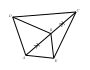
\includegraphics[width = 0.5\textwidth]{Vectors_Assessment_Image_1}

Using the image above, answer yes or no to the following questions. Note that Line segments \(AB\) and \(BC\) are parallel and have equal length which means that \(\pvec{AB} = \pvec{BC}\). If the answer is yes, prove your result using the following algebraic rules:
\begin{itemize}
\item Vector addition is commutative: \(\mvec{u} + \mvec{v} = \mvec{v} + \mvec{u}\)
\item Vector addition is associative: \((\mvec{u} + \mvec{v}) + \mvec{w} = \mvec{u} + (\mvec{v} + \mvec{w})\)   
\item Distributive laws: \((k_1 + k_2)\mathbf{u} = k_1\mathbf{u} + k_2\mathbf{u}\) and \(k(\mathbf{u} + \mathbf{v}) = k\mathbf{u} + k\mathbf{v}\)
\item Head to tail vector addition: Given points \(P\), \(Q\), and \(R\), then \(\pvec{PQ} + \pvec{QR} = \pvec{PR}\)
\item Given points \(P\) and \(Q\), then \(\pvec{QP} = -\pvec{PQ}\)
\end{itemize}


Answer with yes or no the following (include a proof if the answer is yes):
\begin{itemize}
\item Does \(\pvec{BC} + \pvec{CD} = \pvec{BD}\) ~?
\item Does \(\pvec{BD} + \pvec{EB} = \pvec{EA} + \pvec{AD}\) ~?
\item Does \(\pvec{EB} + \pvec{AE} + \pvec{BD} = \pvec{AD}\) ~?
\item Does \(\pvec{AB} + \pvec{AE} = \pvec{BE}\) ~?
\item Does \(\pvec{AB} + \pvec{CB} = \pvec{\mathbf{0}}\) ~?
\item Does \(\pvec{AC} = 2\pvec{AB}\) ~?
\item Does \(\pvec{BC} = \frac{1}{2}\pvec{CA}\) ~?
\end{itemize}

\section*{Question 3}




\end{document}















